\chapter{Finanza Aziendale}
\section{Finanza d'impresa e massimizzazione del valore}
Tutto ciò che riguarda la \textbf{massimizzazione del valore dell'impresa} rientra nelle decisioni finanziarie. L'obiettivo principale della finanza 
aziendale è infatti prendere decisioni che contribuiscano ad aumentare il valore dell'impresa e, di conseguenza, la ricchezza degli azionisti.

\subsection{Concetti fondamentali}
I principali termini utilizzati in finanza sono:
\begin{itemize}
    \item \textbf{Attività reali} $\rightarrow$ beni materiali o immateriali utilizzati dall'impresa per svolgere la propria attività e
    generare valore, come impianti, macchinari, immobili e brevetti;
    \item \textbf{Attività finanziarie} $\rightarrow$ strumenti che rappresentano un diritto sui flussi di cassa futuri, 
    come azioni, obbligazioni e altri titoli;
    \item \textbf{Mercati finanziari e dei capitali} $\rightarrow$ mercati nei quali vengono scambiate attività 
    finanziarie e le imprese possono reperire risorse per finanziare i propri investimenti;
    \item \textbf{Decisioni di investimento (Capital Budgeting)} $\rightarrow$ riguardano la scelta dei progetti e delle attività reali 
    nei quali investire;
    \item \textbf{Decisioni di finanziamento} $\rightarrow$ riguardano il modo in cui reperire le risorse necessarie agli investimenti, ad esempio 
    attraverso capitale proprio o capitale di debito.
\end{itemize}
\noindent Le principali funzioni dei mercati finanziari sono:
\begin{itemize}
    \item \textbf{Finanziamento} $\rightarrow$ permettono alle imprese di raccogliere capitale;
    \item \textbf{Liquidità} $\rightarrow$ permettono agli investitori di acquistare e vendere facilmente attività finanziarie;
    \item \textbf{Determinazione dei valori di mercato} $\rightarrow$ contribuiscono alla formazione del valore di mercato delle imprese e dei titoli.
\end{itemize}
\begin{figure}[H]
    \centering  
    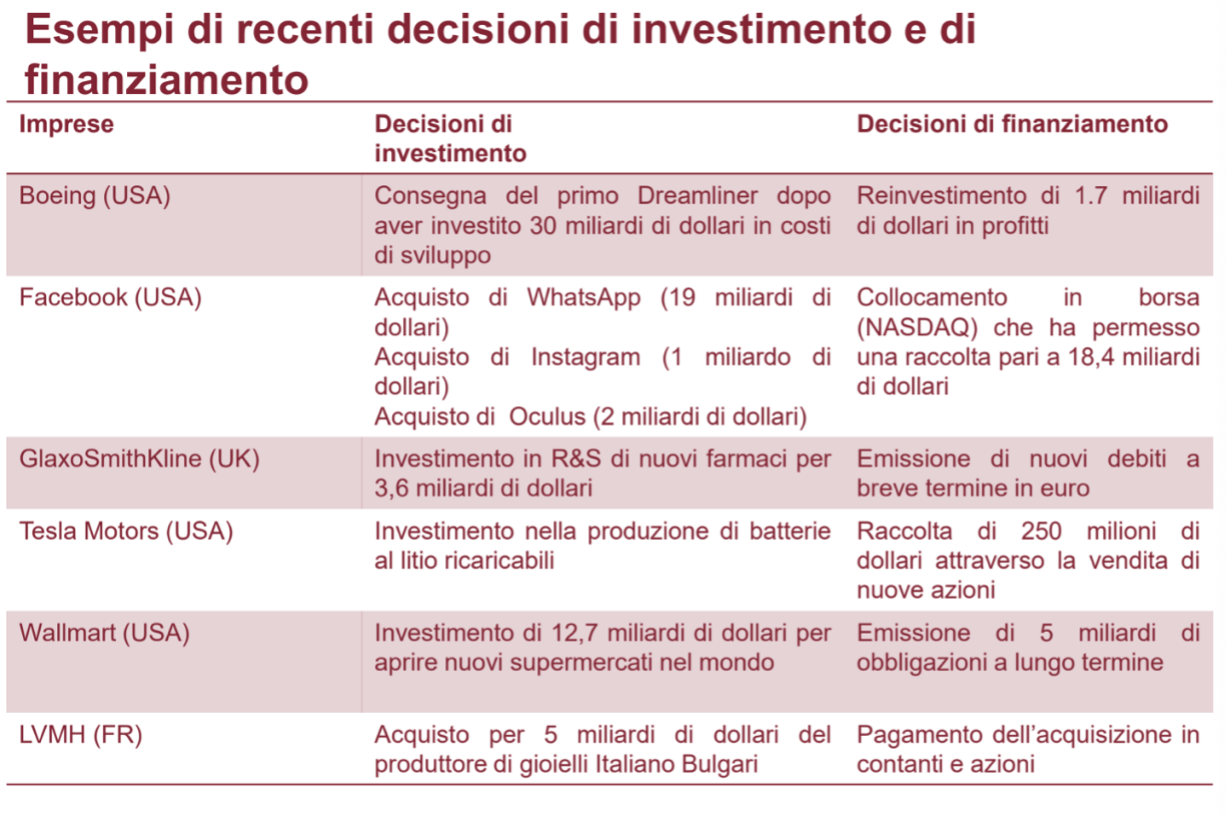
\includegraphics[width=0.6\linewidth]{../images/Esempi Finanziari.png}
    %\label{label}
\end{figure}
\begin{figure}[H]
    \centering  
    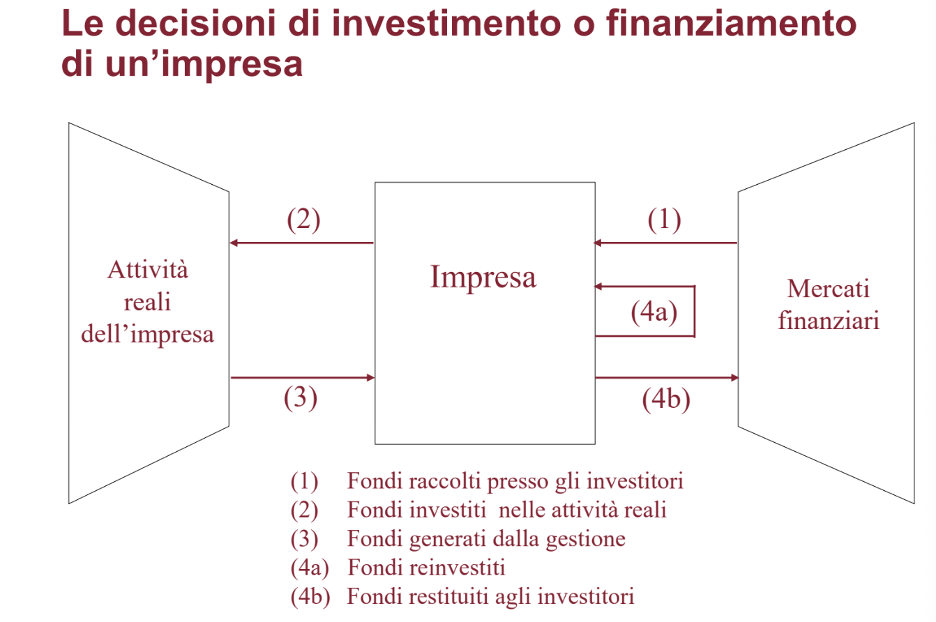
\includegraphics[width=0.8\linewidth]{../images/Decisioni.png}
    \caption{Decisoni finanziarie e flussi di cassa}
    %\label{label}
\end{figure}
\subsection{Rapporto tra impresa e investitori}
Il rapporto tra investitori e impresa può essere suddiviso in tre fasi:
\begin{enumerate}
    \item \textbf{Finanziamento} $\rightarrow$ gli investitori forniscono capitale all'impresa;
    \item \textbf{Investimento} $\rightarrow$ l'impresa utilizza il capitale raccolto per finanziare attività reali e progetti;
    \item \textbf{Rendimento} $\rightarrow$ gli investimenti generano flussi di cassa e quindi un rendimento per gli investitori.
\end{enumerate}

\noindent Gli azionisti finanziano un'impresa solamente se le decisioni di investimento generano un \textbf{rendimento adeguato}, cioè almeno pari al 
rendimento ottenibile attraverso investimenti alternativi presenti sul mercato finanziario caratterizzati dallo stesso livello di rischio.
\begin{figure}[H]
    \centering  
    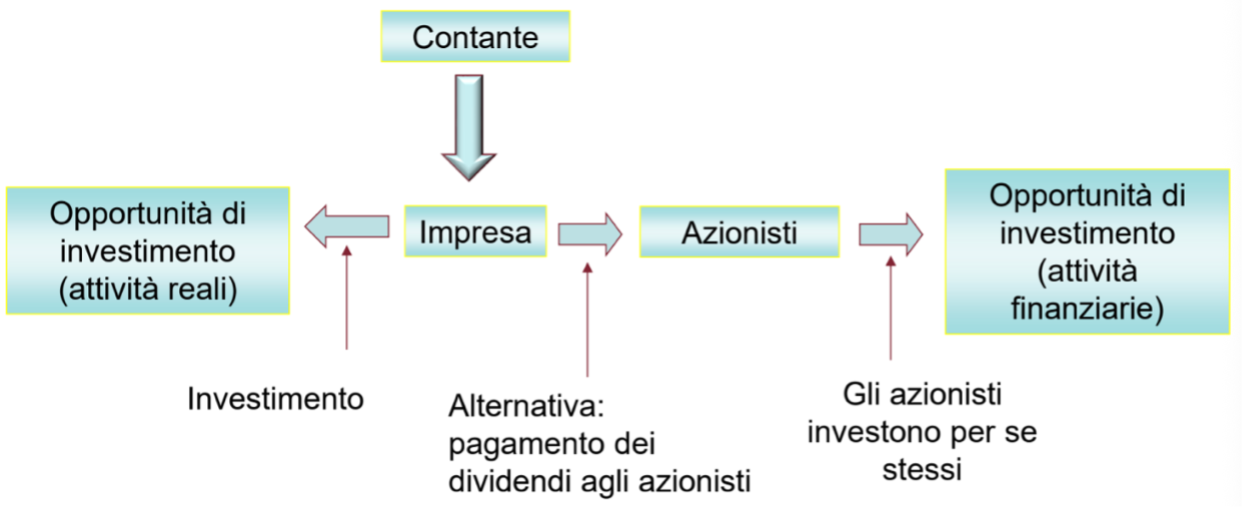
\includegraphics[width=0.9\linewidth]{../images/Trade off.png}
    \caption{Trade-off tra rischio e rendimento}
    %\label{label}
\end{figure}
\subsection{Financial Manager}
Le decisioni di investimento e di finanziamento vengono coordinate dal \textbf{Financial Manager}, responsabile della gestione finanziaria dell'impresa.
Nelle imprese di piccole dimensioni una singola persona può essere responsabile di gran parte delle decisioni strategiche. Nelle imprese più grandi, invece, 
la responsabilità è distribuita tra più soggetti.

\noindent Le decisioni finanziarie non dipendono esclusivamente dal top management. Anche altre figure possono influenzarle: ad esempio, un ingegnere che progetta un nuovo impianto contribuisce a determinare il tipo di attività reale nella quale l'impresa investirà.

\noindent L'\textbf{obiettivo finanziario dell'impresa} è quindi quello di massimizzare il valore di mercato dell'azienda e, indirettamente, aumentare la ricchezza degli azionisti.

\subsection{Separazione tra proprietà e controllo}
Nelle imprese di maggiori dimensioni si verifica generalmente una separazione tra:
\begin{itemize}
    \item \textbf{Proprietà} $\rightarrow$ rappresentata dagli azionisti;
    \item \textbf{Controllo} $\rightarrow$ affidato ai manager che amministrano l'impresa.
\end{itemize}

\noindent Questa separazione presenta vantaggi e svantaggi:
\begin{verbatim}
VANTAGGI:
+ continuità dell'impresa anche in caso di cambiamento dei proprietari
+ gestione affidata a manager professionisti e specializzati

SVANTAGGI:
- possibili obiettivi differenti tra manager e azionisti
- possibili decisioni che non tutelano gli interessi degli azionisti
\end{verbatim}

\noindent Questa situazione dà origine al cosiddetto \textbf{modello principale-agente} o \textbf{modello di agenzia}:
\begin{itemize}
    \item \textbf{Principale} $\rightarrow$ azionisti;
    \item \textbf{Agente} $\rightarrow$ manager.
\end{itemize}

\noindent Gli azionisti affidano ai manager il compito di gestire l'impresa. Tuttavia, gli interessi delle due parti possono essere differenti e i manager potrebbero prendere decisioni che favoriscono i propri interessi invece di quelli degli azionisti.

\noindent Il \textbf{problema di agenzia} rappresenta quindi il possibile conflitto di interessi derivante dalla separazione tra proprietà e controllo.
\begin{figure}[H]
    \centering  
    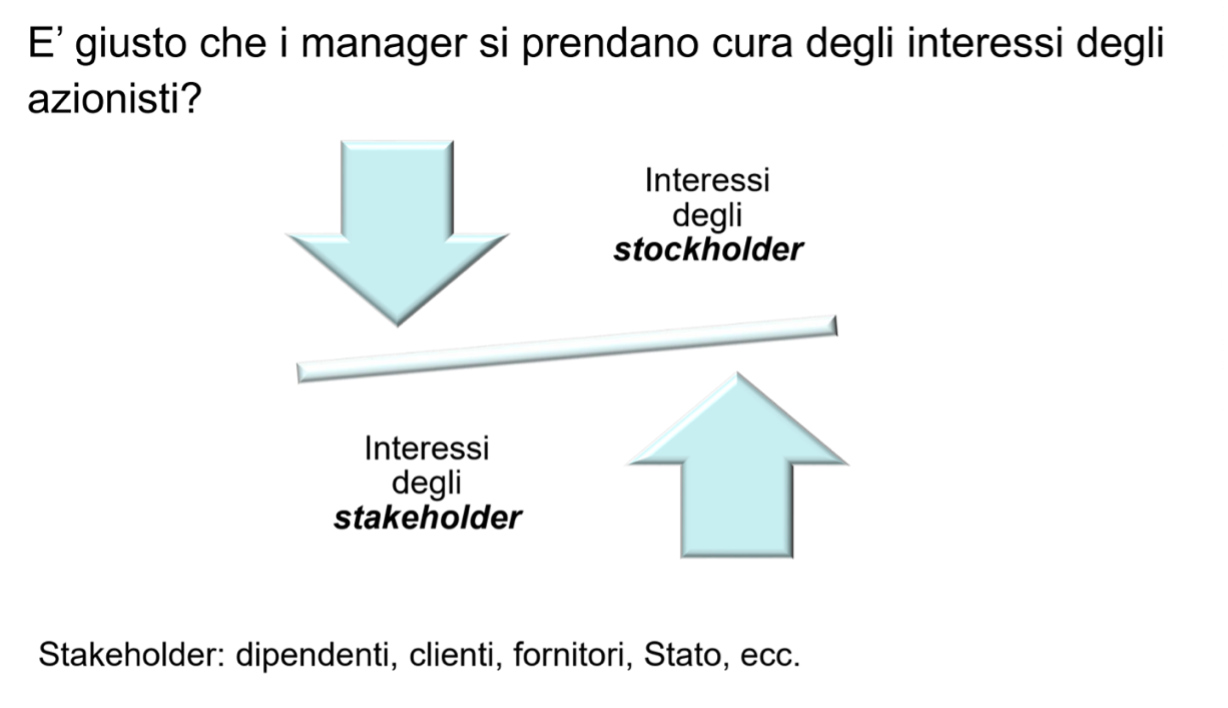
\includegraphics[width=0.5\linewidth]{../images/Stakeholder.png}
    \caption{Stakeholder}
    %\label{label}
\end{figure}
\subsection{Corporate Governance}
La \textbf{Corporate Governance} comprende l'insieme di regole, strutture e meccanismi utilizzati per controllare e indirizzare la gestione dell'impresa, cercando di allineare gli interessi dei manager con quelli degli azionisti.

\noindent Tra i principali meccanismi troviamo:
\begin{enumerate}
    \item \textbf{Consiglio di amministrazione} $\rightarrow$ controlla e valuta l'operato dei manager;
    \item \textbf{Sostituzione del management} $\rightarrow$ manager inefficienti possono essere sostituiti con manager più efficienti;
    \item \textbf{Incentivi finanziari} $\rightarrow$ strumenti come bonus e stock option collegano la remunerazione dei manager ai risultati dell'impresa.
\end{enumerate}

\noindent Le principali soluzioni al problema di agenzia sono:
\begin{itemize}
    \item piani di remunerazione e incentivazione;
    \item controllo da parte del consiglio di amministrazione;
    \item scalate ostili (\textit{hostile takeovers});
    \item monitoraggio da parte degli analisti finanziari;
    \item pressione e controllo esercitati dagli azionisti.
\end{itemize}

\noindent In sintesi, gli azionisti mirano alla \textbf{massimizzazione del valore dell'impresa}, ma non è necessariamente garantito che i manager perseguano sempre lo stesso obiettivo. I meccanismi di Corporate Governance cercano quindi di ridurre il problema di agenzia e allineare gli interessi delle due parti.